\chapter{Strahlverfolgung}\label{ch:strahlerzeugung}

Die rudimentäre Funktionsweise eines "`Raytracers"' besteht darin, Strahlen in eine Szene, bestehend aus Objekten und Lichtquellen, auszusenden und zu überprüfen, ob diese ein Objekt treffen. Im Falle eines Schnittes wird die Schattierung des Objekts am Strahl-Objekt Schnittpunkt berechnet und diese Information wird entlang des Strahls auf eine Projektionsebene zurück propagiert. In Kapitel~\ref{ch:schattierung} wird die genaue Vorgehensweise zur Schattierungsberechnung erläutert.

In diesem Kapitel wird es darum gehen, die grundlegenden Komponenten vorzubereiten, die es dem "`Raytracer"' ermöglichen, Strahlen in eine Szene auszusenden.
Dazu benötigt man eine geeignete Repräsentation eines Strahls sowie ein Kameramodell, welches die Ansicht der Szene bestimmt. Die vom Kameramodell erzeugten Strahlen werden auch Primärstrahlen genannt. Im folgenden werden zwei Kameramodelle vorgestellt und zwar in Form einer orthografische Kamera und in Form einer Lochkamera.

Die Besonderheit besteht bei der orthografischen Kamera darin, dass die Strahlen parallel zueinander verlaufen (s. Abb~\ref{fig:orthocam}). Diese Art der Projektion wird häufig in technischen Zeichnungen verwendet, da Objekte nicht kleiner dargestellt werden, wenn sie sich von der Projektionsebenen entfernen, und somit ein besserer Vergleich der Größe von Objekten gegeben ist.

Die Lochkamera sorgt für eine perspektivische Projektion der Objekte auf die Projektionsebene. Dadurch erscheinen Objekte kleiner je weiter sie vom Beobachter entfernt sind (s. Abb~\ref{fig:pers_proj}).



\begin{minipage}[t]{0.43\textwidth}
    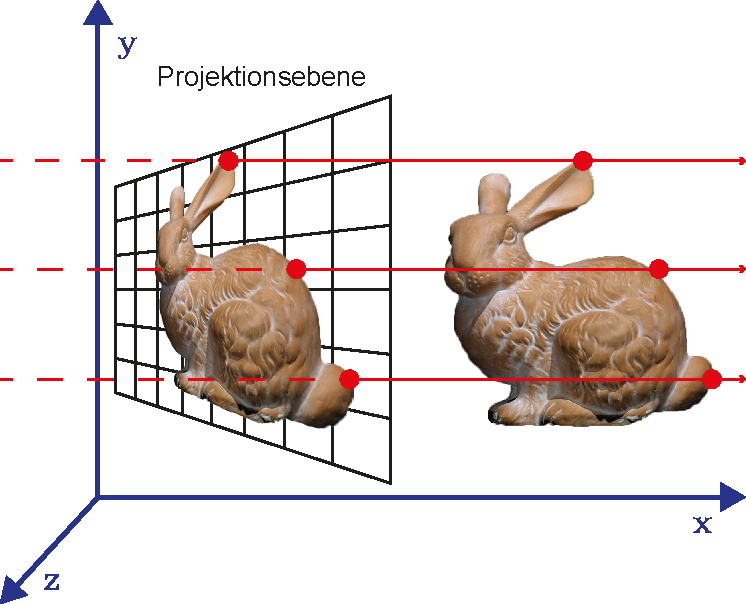
\includegraphics[width=\textwidth]{./img/strahlverfolgung/orth_proj.pdf}
    \captionof{figure}{Orthografische Kamera}
    \label{fig:orthocam}
\end{minipage}
\begin{minipage}[t]{0.51\textwidth}
    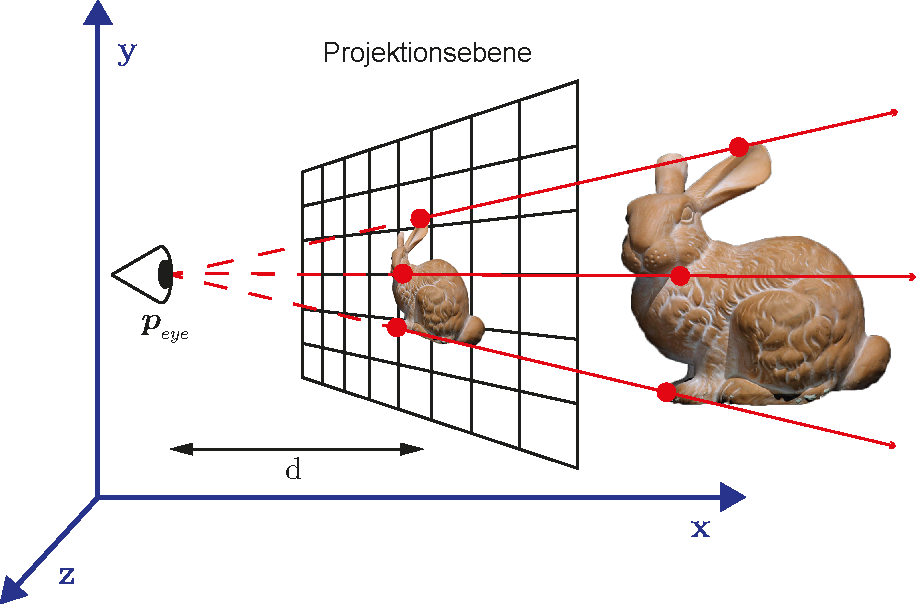
\includegraphics[width=\textwidth]{./img/strahlverfolgung/pers_proj.pdf}
    \captionof{figure}{Lochkamera}
    \label{fig:pers_proj}
\end{minipage}




\section{Strahlgleichung}

Ein Strahl besitzt die folgende parametrisierte Form:
\begin{equation}
\label{eq:Strahlgleichung}
\boldsymbol{r} = \boldsymbol{o} + t \cdot \boldsymbol{d}
\end{equation}

Der Punkt $\boldsymbol{o}$ ist der Ursprung des Strahls. Die Strahlrichtung ist durch den Vektor \( \boldsymbol{d} \) gegeben.
Der Parameter \( t \) kann beliebig gewählt werden und wird später dazu verwendet den Schnittpunkt $\boldsymbol{r}$ eines Strahls mit einem Objekt zu berechnen.

Um nun einen Strahl in eine Szene auszusenden, genügt es, seinen Ursprung \( \boldsymbol{o} \) sowie  Richtung \( \boldsymbol{d} \) festzulegen. Dies ist die Aufgabe des 
Kameramodells.


\section{Projektionsebene}

\begin{wrapfigure}[18]{r}{0.45\textwidth}    
    \vspace{-15pt}
    \centering
    
\includegraphics[width=0.44\textwidth]{./img/strahlverfolgung/projektionsebene}
    \vspace{-10pt}
    \caption{Die Projektionsebene mit Höhe $ h $, Breite $b$, Mittelpunkt $\boldsymbol{p}_{proj}$, "`Up-Vektor"' $\boldsymbol{u}_{proj}$ und Normale $\boldsymbol{n}_{proj}$. Sie ist unterteilt in gleichgroße Quadrate (PEE) mit Kantenlänge $l_{PEE}$.}
    \label{fig:projektionsebene}   
\end{wrapfigure}

Die Projektionsebene ist ein essentieller Bestandteil der nachfolgenden Kameramodelle. Tatsächlich handelt sich dabei nicht um eine Ebene, sondern um eine rechteckige Fläche mit der Höhe \( h \) und der Breite \( b \). Sie ist in kleinere Projektionsebenen-Elemente (PEE\abk{PEE}{Projektionsebenen-Elemente}) unterteilt, die nichts weiter als Quadrate   gleicher Größe sind. PEE besitzen die Kantenlänge \( l_{PEE} \). Es erweist sich als praktisch, die Größe bzw. das Seitenverhältnis der Projektionsebene festzulegen und anschließend anhand der Kantenlänge der PEE Einfluss auf die Auflösung des fertigen Bildes zu nehmen.
Denn zum Ende der Bildsynthese enthalten die PEE Farbwerte, die auf Bildelemente eines Ausgabemediums übertragen werden können. Im Falle des Monitors besteht eine einfache Abbildung darin, den Farbwert eines PEE durch genau einen Bildpunkt des Monitors ausgeben zu lassen.



\section{Orthografische Kamera}

Das Prinzip der orthografischen Kamera ist recht simpel, daher eignet sie sich ausgezeichnet, um die korrekte Funktionsweise des "`Raytracers"' zu Beginn der Implementationsphase zu überprüfen.

Sie besteht aus einer Projektionsebene (s. Abb. \ref{fig:projektionsebene} ), die innerhalb des globalen Koordinatensystems eine Position \( \boldsymbol{p}_{proj} \) und eine Ausrichtung besitzt, die durch die Normale \( \boldsymbol{n}_{proj} \) und einem "`Up-Vektor"' \( \boldsymbol{u}_{proj} \) gegeben ist. Das Ziel besteht nun darin, Strahlen durch die einzelnen PEE hindurch in die Szene zu schicken. Trifft ein Strahl auf ein Objekt, wird am Schnittpunkt die Schattierung berechnet und diese Information dem PEE zugeordnet, welches vom entsprechenden Strahl durchdrungen wurde. 

Zur Erzeugung der Strahlen empfiehlt es sich die Projektionsebene zu Beginn so zu positionieren, dass sich ihr Mittelpunkt im Ursprung des globalen Koordinatensystems befindet. 
Ihre Normale zeigt in die der z-Achse entgegengesetzte Richtung und der "`Up-Vektor"' verläuft parallel zur y-Achse. Man kann nun relativ leicht den Mittelpunkt der einzelnen PEE berechnen. Dieser dient jeweils als Strahlursprung. Die Richtung der Strahlen verläuft parallel zur z-Achse und zwar in negativer Richtung.
Die Position und Richtung der so erzeugten Strahlen werden mit \( \boldsymbol{o'} \) und \( \boldsymbol{d'} \) bezeichnet.

Diese Strahlen müssen nun vom globalen ins Kamera lokale Koordinatensystem transformiert werden. Dies gelingt, indem man eine Orthonormalbasis (ONB\abk{ONB}{Orthonormalbasis}) aus \( \boldsymbol{n}_{proj} \) und \( \boldsymbol{u}_{proj} \) erzeugt, dann einen Basiswechsel durchführt und anschließend um den Vektor \( \boldsymbol{v} = \boldsymbol{p}_{proj} - \begin{pmatrix} 0 & 0 & 0 & 1 \end{pmatrix}^\intercal \) verschiebt.

Es sei vorausgesetzt, dass:

\begin{equation*}
|\boldsymbol{n}_{proj}| = 1; \qquad |\boldsymbol{u}_{proj}| = 1; \qquad \boldsymbol{n}_{proj} \cdot \boldsymbol{u}_{proj} = 0 
\end{equation*}

dann ist die ONB gegeben durch:

\begin{equation}
    \boldsymbol{e}_1 = \boldsymbol{n}_{proj} \times \boldsymbol{u}_{proj}; \qquad \boldsymbol{e}_2 = \boldsymbol{u}_{proj}; \qquad \boldsymbol{e}_3 = -\boldsymbol{n}_{proj}
    \label{eq:onb}
\end{equation}

Basiswechsel durchführen mit:

\begin{align}
    \boldsymbol{o''} &= \boldsymbol{o'}.x \cdot \boldsymbol{e}_1 + \boldsymbol{o'}.{y} \cdot \boldsymbol{e}_2 + \boldsymbol{o'}.{z} \cdot \boldsymbol{e}_3 + 
                      \boldsymbol{o'}.{w} \cdot \begin{pmatrix} 0 & 0 & 0 & 1 \end{pmatrix}^\intercal \\
    \boldsymbol{d}         &= \boldsymbol{d'}.{x} \cdot \boldsymbol{e}_1 + \boldsymbol{d'}.{y} \cdot \boldsymbol{e}_2 + \boldsymbol{d'}.{z} \cdot \boldsymbol{e}_3 \label{eq:onb_richtung}
\end{align}

wobei \( \boldsymbol{o'}.{x}, \boldsymbol{d'}.{x}, \dots, \boldsymbol{d'}.w\) usw. die jeweilige Komponente von \( \boldsymbol{o'} \) und \( \boldsymbol{d}' \) bezeichnet.
Anschließend um den Vektor \( \boldsymbol{v} \) verschieben.

\begin{equation*}
    \boldsymbol{o} = \boldsymbol{o''} + \boldsymbol{v}
\end{equation*}

Im Fall der orthografischen Kamera kann Gleichung~\ref{eq:onb_richtung} entfallen, da aufgrund des senkrechten Austrittswinkel der Strahlen aus der Projektionsebene einfach \( \boldsymbol{d} = \boldsymbol{n}_{proj} \) gesetzt werden kann.


\section{Lochkamera}

Bei realen Lochkameras werden Objekte an der Lochblende um \( 180^\circ \) gedreht auf einen Film oder Sensor abgebildet. Dieser Umstand lässt sich beim virtuellen Kameramodell gut vermeiden, indem man den Betrachter an die Position der Lochblende setzt und ihn auf die Szene richtet. Die Projektionsebene nimmt die Rolle des Films ein und wird zwischen Betrachter und Szene eingebracht. Je kleiner das Loch ist, desto schärfer wird das Bild in der Realität, da störende Randstrahlen abgeschirmt werden.

Die Position des Betrachters \( \boldsymbol{p}_{eye} \) dient als Startpunkt für die Strahlen und kann als unendlich kleines Loch angesehen werden, wodurch maximal scharfe Bilder erzeugt werden. Bei der orthografischen Kamera spielt es generell keine Rolle, ob der Startpunkt der Strahlen auf der Projektionsebenen liegt oder irgendwo davor. Bei der Lochkamera verhält es sich komplett anders. Die Entfernung des Betrachters, in Abb.~\ref{fig:pers_proj} mit \( d \) gekennzeichnet, entscheidet nämlich darüber, wie groß das Sichtfeld ausfällt. Durch folgende Formel lässt sich \( d \) bestimmen:

\begin{equation*}   
     d = \frac{b}{2 \cdot \tan{(\phi_{hfov} \cdot \frac{1}{2})}}
\end{equation*}

\( b \) ist die Breite der Projektionsebene.
\( \phi_{hfov} \) ist der Winkel, der zwischen \( \boldsymbol{p}_{eye} \) und Mittelpunkt der Projektionsebene, sowie \( \boldsymbol{p}_{eye} \) und Mittelpunkt der seitlichen Kante der Projektionsebene aufgespannt wird. Das Sichtfeld des Menschen beträgt fast \( 180^\circ \), was im Bogenmaß einem \( \phi_{hfov} \) von \( \pi \) entsprechen würde. Da der Monitor jedoch nur einen Teil des menschlichen Sichtfelds einnimmt, hat sich ein Wert von \( \frac{\pi}{2} \) für \( \phi_{hfov} \) als geeignet herausgestellt.

Um Strahlen zu erzeugen, richtet man die Projektionsebene wie bei der orthografischen Kamera gezeigt aus, d.h. im Mittelpunkt des globalen Koordinatensystems und die Normale in Richtung negativer z-Achse. Der Betrachter  wird an Position \( \boldsymbol{p}_{eye} \) = \( \begin{pmatrix} 0 & 0 & d & 1 \end{pmatrix}^\intercal \) gesetzt. Sei \( \boldsymbol{m}_{PEE} \) der Mittelpunkt eines PEE, dann ergibt sich die vorläufige Richtung \( \boldsymbol{d'} \) eines Strahls aus \( \boldsymbol{d'} = \boldsymbol{m}_{PEE} - \boldsymbol{p}_{eye} \). Anschließend erzeugt man eine ONB nach Gleichung~\ref{eq:onb} und berechnet die endgültige Strahlrichtung \( \boldsymbol{d} \), wie in \ref{eq:onb_richtung} gezeigt. Für den Strahlursprung lässt sich einfach \( \boldsymbol{o} = \boldsymbol{p}_{eye}\) setzen.


